% Created 2023-08-30 ons 18:21
% Intended LaTeX compiler: pdflatex
\documentclass[11pt]{article}
\usepackage[utf8]{inputenc}
\usepackage[T1]{fontenc}
\usepackage{graphicx}
\usepackage{grffile}
\usepackage{longtable}
\usepackage{wrapfig}
\usepackage{rotating}
\usepackage[normalem]{ulem}
\usepackage{amsmath}
\usepackage{textcomp}
\usepackage{amssymb}
\usepackage{capt-of}
\usepackage{hyperref}
\author{Nadim}
\date{\today}
\title{}
\hypersetup{
 pdfauthor={Nadim},
 pdftitle={},
 pdfkeywords={},
 pdfsubject={},
 pdfcreator={Emacs 27.1 (Org mode 9.3)}, 
 pdflang={English}}
\begin{document}

\tableofcontents

\section{TDP028}
\label{sec:orgb3b8bf9}

\section{Navigering}
\label{sec:orgb021ef4}
\begin{itemize}
\item\relax [Appbeskrivning](\#Appbeskrivning)
\item\relax [Konkurrensanalys](\#Konkurrensanalys)
\end{itemize}

\section{Appbeskrivning}
\label{sec:org923a981}

Kärnpoängen med "Focus \& Fun" är att förbättra fokus under studierna,
arbetet eller programmeringssessioner. Men också att ha lite kul efter
en intensiv session. Appen introducerar "fokusläge" som kommer att
blockera de flesta interaktioner med telefonen förutom nödsamtal. För
varje minut som användaren spenderar i "fokusläge". Hen kommer att få
en "fokuspoäng" helt enkelt kallas FP. Varje 60 fp användaren kan få
en kista med slumpmässiga utmaningar. Dessa utmaningar är utformade
för att förlänga fokustiden eller till ge någon hälsosam
aktivitet/utmaning.

När en kista öppnas kan användaren bestämma om han vill göra
utmåning/aktivitet eller ej.

Några av utmaningarna kan se ut så här:
\begin{itemize}
\item 2 gånger på nästa fokussession
\item +15/30/45m till nästa fokuspass
\end{itemize}

Vissa aktiviteter kan se ut så här:

\begin{itemize}
\item Gå en promenad på 15 m
\item Läs En Bok I 15m
\end{itemize}

Appen kommer inte att ha ett bestraffningssystem samt en kontroll om
användaren har utfört en aktivitet eller inte. Det är bara roligt,
hälsosamt och effektivt.

\section{Konkurrensanalys}
\label{sec:orgec9fb38}

I denna konkurrentanalys kommer appen "Forest: Focus for Productiv-
ity" att analyseras. Appen finns på App store och Google Play Store. App
Store-versionen av appen är ej gratis. Denna app är gjord för att "Hålla
fokus genom att plantera träd!".
Denna applikation valdes på grund av ganska stora utbud av funktioner,
en unik idé med enkel design, ett stort antal positiva recensioner i Google
Play Store samt möjligheten att plantera riktiga träd genom att hålla fokus.

\begin{itemize}
\item Måste-krav
\begin{itemize}
\item En användare ska kunna ställa in tidsintervallet för fokussessionen.
\item En användare ska inte kunna gå ur fokusläge eller öppna andra appar som inte är nödsituationer.
\item En användare ska kunna avsluta fokussessionen.
\item En användare ska kunna få poäng för varje n tid som spenderas i fokusläge.
\item En användare ska kunna spendera intjänade poäng.
\end{itemize}

\item Egna-krav
\begin{itemize}
\item En användare ska kunna få slumpmässiga utmaningar eller aktiviteter.
\item En användare ska kunna sätta kort pause på focus session vid behöv.
\item En användare ska kunna tacka nej till utmåning eller aktivitet.
\item En användare ska kunna se egen utmåning och aktivitets statistik.
\end{itemize}

\item Ux-bilder
\begin{center}
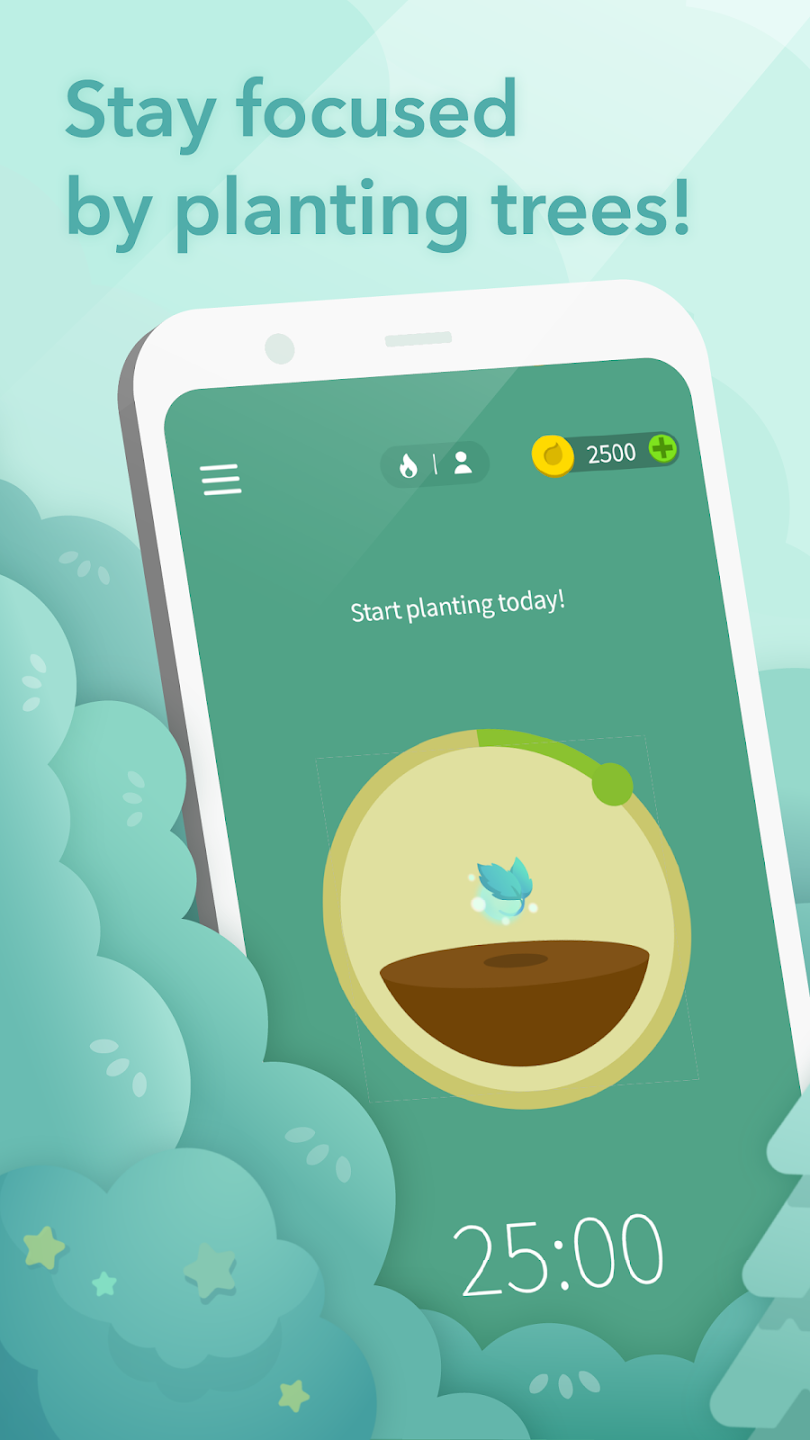
\includegraphics[width=.9\linewidth]{./docs/1.png}
\end{center}
\begin{center}
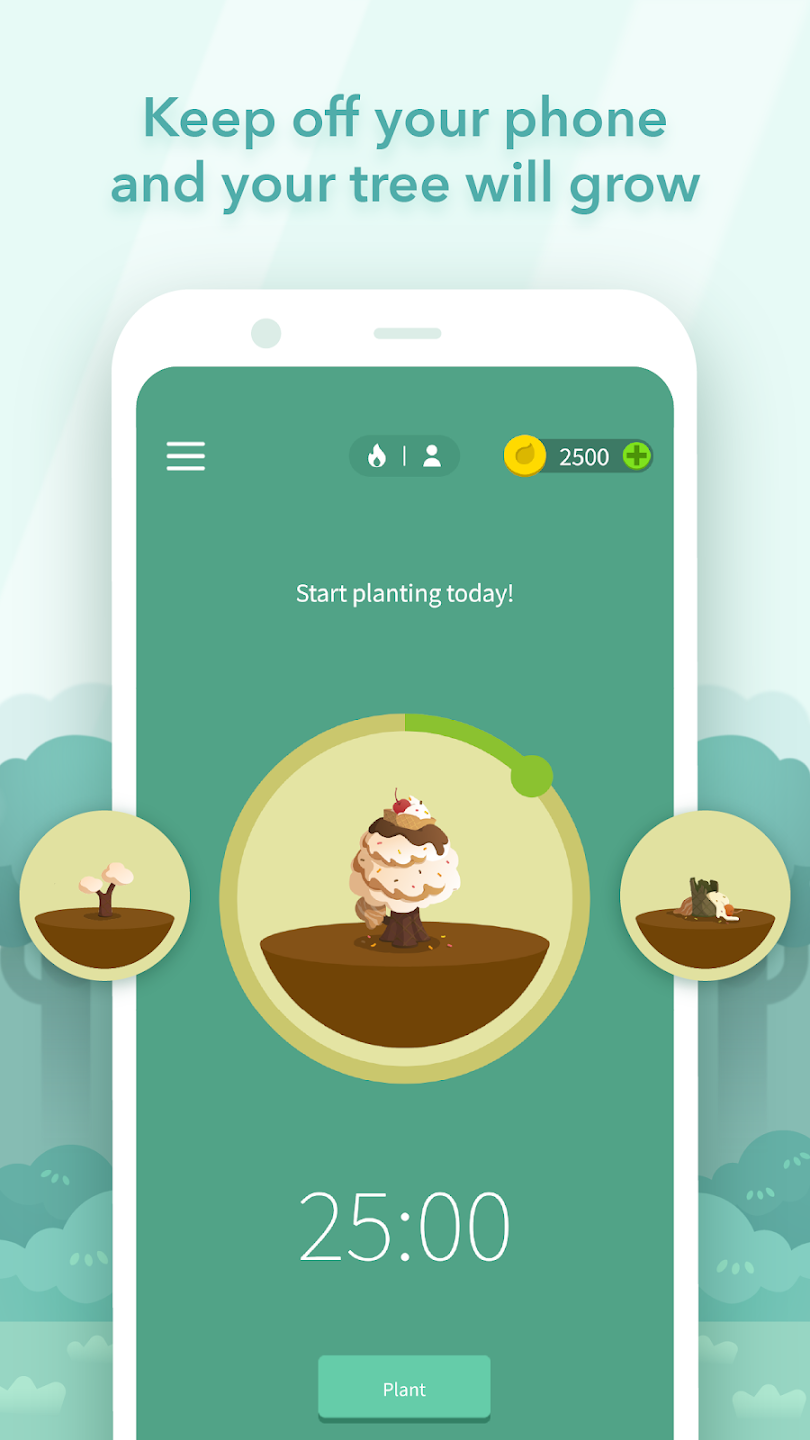
\includegraphics[width=.9\linewidth]{./docs/2.png}
\end{center}
\begin{center}
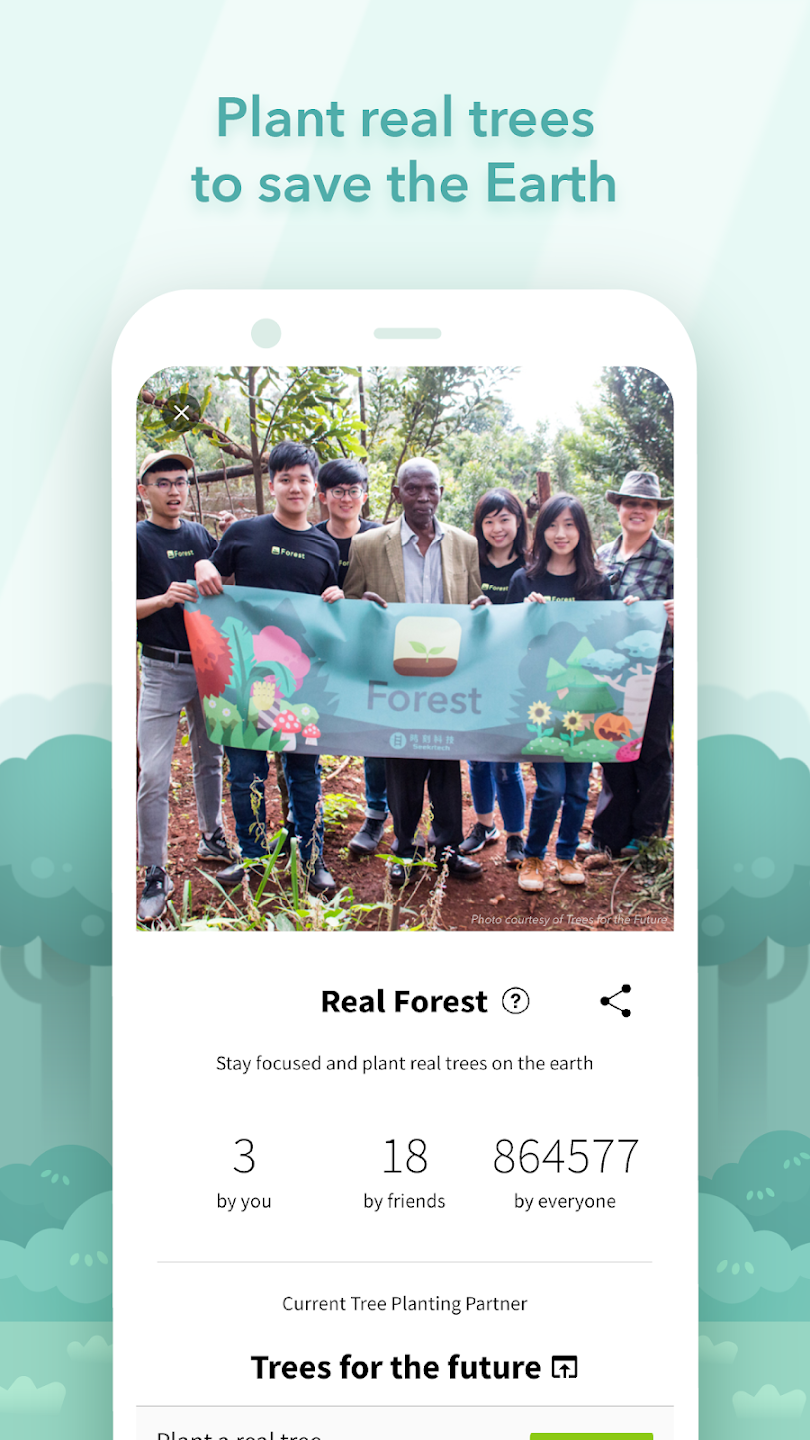
\includegraphics[width=.9\linewidth]{./docs/3.png}
\end{center}
\begin{center}
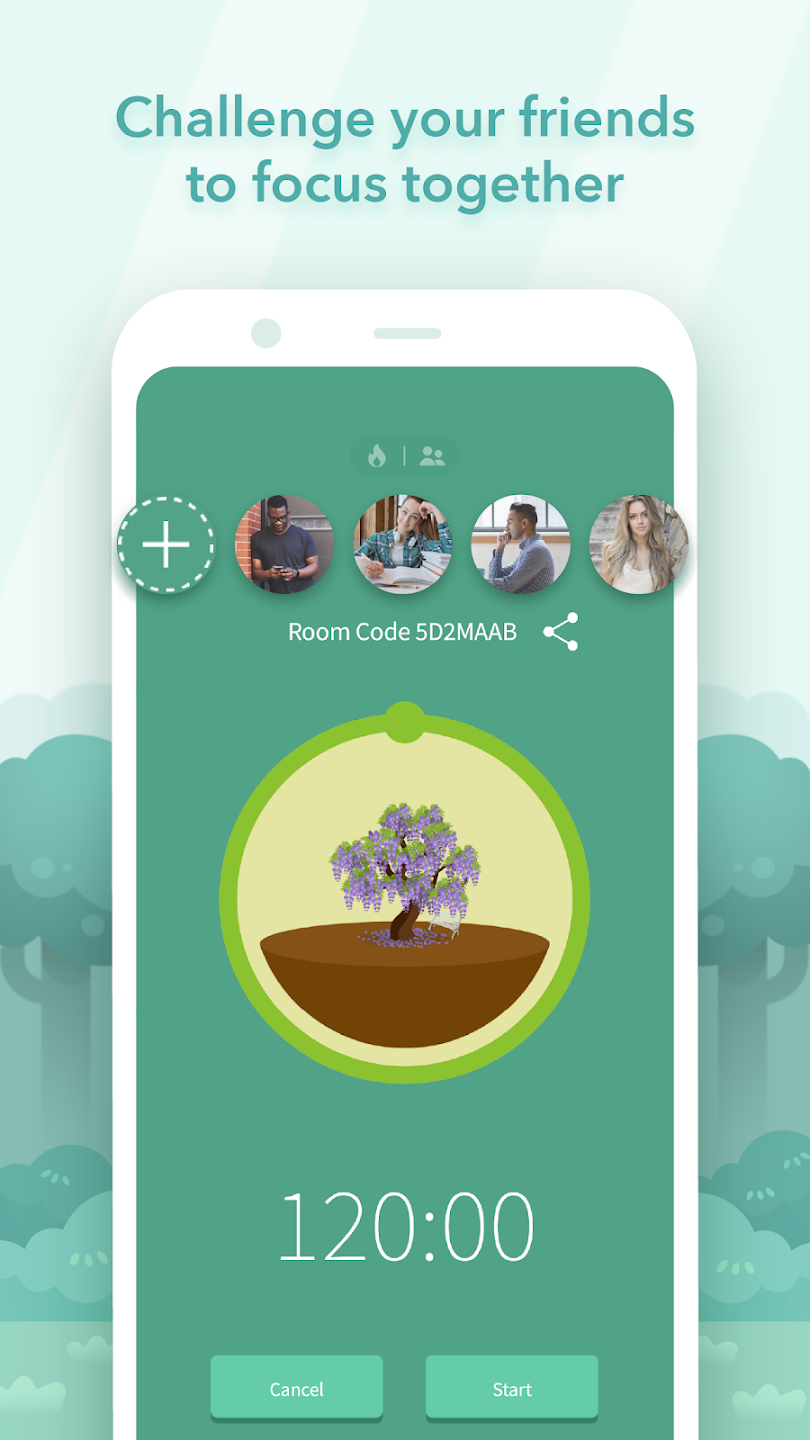
\includegraphics[width=.9\linewidth]{./docs/4.png}
\end{center}
\end{itemize}
\end{document}
